\documentclass{report}
\usepackage{enumitem}
\usepackage{amsmath}
\usepackage{booktabs}
\usepackage{fancyhdr}
\usepackage{tikz}
\usetikzlibrary{calc,positioning,shapes.multipart,shapes}
\usepackage[margin=1in]{geometry}

\renewcommand{\it}[1]{\textit{{#1}}}
\renewcommand{\bf}[1]{\textbf{{#1}}}
\renewcommand{\tt}[1]{\texttt{{#1}}}

\newcommand{\ib}[1]{\it{\bf{{#1}}}}

\pagestyle{fancy}
\fancyhf{}

\fancyhead[L]{\bf{Computer Science 143}}
\fancyhead[C]{\it{Homework 1}}
\fancyhead[R]{\bf{Warren Kim}}
\setlength{\headsep}{0.1in}

\tikzset{
    basic/.style={
        draw,
        rectangle split,
        rectangle split parts=2,
        rectangle split part fill={blue!20,white},
        minimum width=2.5cm,
        text width=2cm,
        align=left,
        font=\itshape
    }
}

\begin{document}
\paragraph{Part 1. Keys}\mbox{} \vspace{10pt}

\noindent Below is a relation $R$ containing attributes $A, B, C$.
\begin{center}
    \begin{tabular}{c|c|c}
        A & B & C \\
        \hline
        $\alpha$ & $\delta$ & $\xi$ \\
        $\beta$ & $\delta$ & $\psi$ \\
        $\gamma$ & $\eta$ & $\xi$
    \end{tabular}
\end{center}

\begin{enumerate}[label=(\alph*)]
    \item Identify all superkeys of $R$. \vspace{2pt}

        \bf{Response:} $\{A, AB, BC, ABC\}$

    \item Identify all candidate keys of $R$. \vspace{2pt}

        \bf{Response:} $\{A, BC\}$
\end{enumerate}

\noindent Below is a relation called \tt{Employee} containing some data about student employees at UCLA 
Recreation. The EmployeeID is created and controlled by UCLA Recreation and is always used 
by only one employee at a time, and is retired (never re-used) after an employee leaves the 
department. Each student employee also has a UID issued by the University.

\begin{table}[h!]
    \centering
    \begin{tabular}{|c|c|c|c|}
        \hline
        \hline
        EmployeeID ($A$) & EmployeeName ($B$) & UID ($C$) & ManagerID ($D$) \\
        \hline
        1 & John Smith  & 123456789 & 9 \\
        \hline
        2 & Sarah Decker & 242424246 & 3 \\
        \hline
        3 & John Smith  & 987654321 & 9 \\
        \hline
        4 & Jane Allison & 112358132 & 1 \\
        \hline
        \hline
    \end{tabular}
\end{table}

\noindent Below is a relation called \tt{Facility} containing data about recreation facilities 
and who manages each one. Each manager has an ID number that has the same format as the 
EmployeeID. A matter of fact, a ManagerID \it{is} an EmployeeID. The primary key of 
this relation is Facility ($A$).

\begin{table}[h!]
    \centering
    \begin{tabular}{|c|c|}
        \hline
        \hline
        Facility ($A$) & ManagerID ($B$) \\
        \hline
        Wooden Center & 1 \\
        \hline
        Sunset Canyon & 3 \\
        \hline
        Drake Stadium & 9 \\
        \hline
        \hline
    \end{tabular}
\end{table}

\begin{enumerate}[label=(\alph*)]
    \setcounter{enumi}{2}
    \item Identify all candidate keys of \tt{Employee} in this instance. \vspace{2pt}

        \bf{Response:} $\{A, C\}$

    \item Based on your answer from part (c), what is the full set of superkeys for
        \tt{Employee} in this instance and why? \it{Be careful}. Explain. \vspace{2pt}

        \bf{Response:} $\{A, C, AB, AC, AD, BC, CD, ABC, BCD, ABCD\}$. The candidate keys of \tt{Employee} are
        $\{A, C\}$ so all supersets of $A, C$ are superkeys.

    \item Which attribute or set of attributes would you choose to be the primary key of 
        \tt{Employee} in this instance and why? \it{Be careful}. Explain. \vspace{2pt}

        \bf{Response:} EmployeeID, because it is the minimal candidate key and enforced to
        be unique by the problem statement (EmployeeID is always used by only one employee at a time 
        and is retired (never re-used) after an employee leaves the department).


    \item Suppose an analyst decides to choose both \tt{EmployeeID} and \tt{UID} 
        as a composite primary key for \tt{Employee} since both are unique. Explain why 
        this is not correct. \bf{Hint:} Think about what this might imply about each 
        attribute in the primary key and what data integrity issues can arise. \vspace{2pt}

        \bf{Response:} This is not correct because the primary key is supposed to be a candidate key, 
        but since EmployeeID and UID are candidate keys by by themselves, the provided composite 
        primary key is, by definition, not a candidate key and therefore not a valid primary key. 

    \item Identify all foreign keys in context of the problem (assume that all tables have more 
        rows). How do these foreign keys help us ensure referential integrity in this context? Note 
        that there may be more than you initially believe. \vspace{2pt}

        \bf{Response:} Let $\cal{E}, \cal{F}$ be the relations for \tt{Employee}, \tt{Facility} 
        respectively. Then $D \in \cal{E}$ and $B \in \cal{F}$ are foreign keys into $A \in \cal{E}$.
        By the problem statement, a ManagerID \it{is} an EmployeeID. Therefore, we ensure referential
        integrity because if we reference a ManagerID $\alpha$ in either relation, the employee 
        with EmployeeID $\alpha$ must exist in \tt{Employee}.
\end{enumerate}

\newpage
\paragraph{Part 2. Schema Diagram}
Suppose you are working for the data team at Starship, a San Francisco based startup that aims to 
revolutionize food delivery. How the Starship service works: a user installs an app on their phone 
and places an order at a participating restaurant within a geofenced region (e.g. UCLA campus). The 
user enters their credit card information, orders their meal and selects where they want the food 
delivered. A code is provided so that only the correct user can open the lid and retrieve their 
food. Due to limited supplies of robots, and high demand, the company wants to experiment with 
charging users based on the amount of time it takes to deliver the food from the restaurant to the 
user. \vspace{10pt}

\noindent We have the following relations for managing robots, users and orders:
\small{
\begin{verbatim}
Robot(robot_id, is_online)
# robot_id is some value that identifies a robot.
# is_online just indicates whether or not the robot is able to be used.

User(user_id, ccnum, expdate, email, name)
# user_id is some value that identifies the user
# ccnum is the user's credit card number (hashed, hopefully!) and may be null, and may change.
# expdate is the credit card expiration date and may also be null, and may change.
# email is the user's email address.
# name is the, well, user's name

Order(order_id, user, robot, restaurant, deliver_lat, deliver_lon, start_time, end_time)
# order_id is some value that identifies the order.
# user uniquely identifies the user that placed the order.
# robot uniquely identifies the robot that delivered the user's food.
# restaurant identifies where the user ordered food.
# deliver_lon is the longitude of the delivery location
# deliver_lat is the latitude of the deliver location
# start_time and end_time represent the start and end times of the delivery.
# we will ignore the details of the order for now.

Restaurant(restaurant_id, name, region)
# restaurant_id is some value that identifies the restaurant.
# name is the name of the restaurant
# region is the name of the geofenced region where the restaurant is located (e.g. UCLA)
\end{verbatim}
}
\noindent \it{Hint:} There is a lot written above; however, remember that we are interested in 
\bf{keys}. \vspace{10pt}

\noindent \bf{Exercise.} Using these relations, draw the schema diagram. For an example of a schema 
diagram, see Figure 2.8 in the text (page 47), or the end of the Intro to the Relational Model 
section in the lecture slides for Lecture 2. Clearly denote primary and foreign keys (note that 
primary keys were intentionally withheld in the specification above).

\begin{center}
    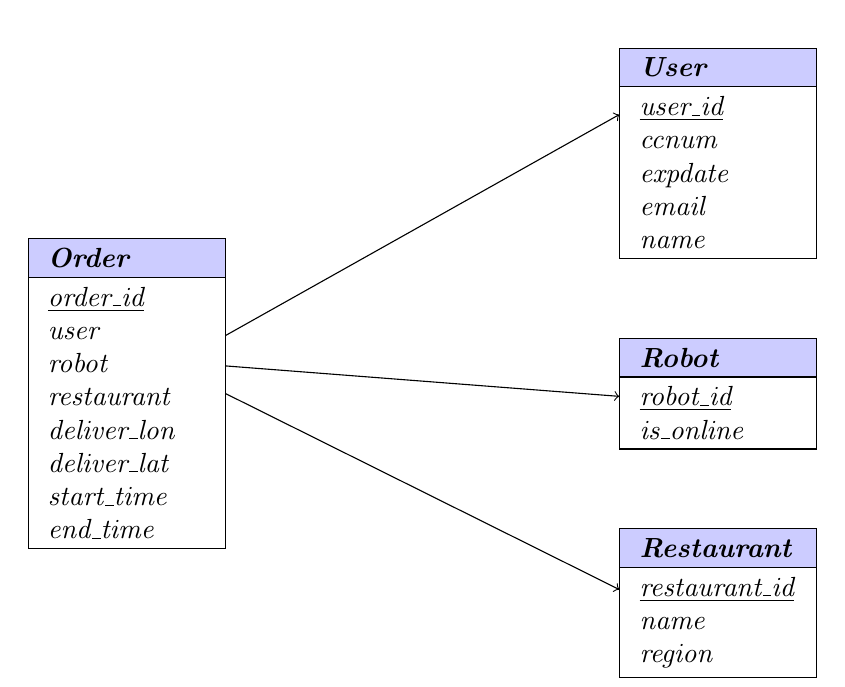
\begin{tikzpicture}
        \node[basic] (Order) {
                \bf{Order}
                \nodepart{second}
                    \underline{order\_id}
                    \newline
                    user
                    \newline
                    robot
                    \newline
                    restaurant
                    \newline
                    deliver\_lon
                    \newline
                    deliver\_lat
                    \newline
                    start\_time
                    \newline
                    end\_time
                };


            \node[basic,right=5cm of Order] (Robot) {
                    \bf{Robot}
                    \nodepart{second}
                        \underline{robot\_id}
                        \newline
                        is\_online
                    };

                \node[basic,above=1cm of Robot] (User) {
                        \bf{User}
                        \nodepart{second}
                            \underline{user\_id}
                            \newline
                            ccnum
                            \newline
                            expdate
                            \newline
                            email
                            \newline
                            name
                        };

                    \node[basic,below=1cm of Robot] (Restaurant) {
                            \bf{Restaurant}
                            \nodepart{second}
                                \underline{restaurant\_id}
                                \newline
                                name
                                \newline
                                region
                            };
                        \draw[->] ([yshift=21pt]$(Order.east)$) -- ([yshift=14pt]$(User.west)$);
                        \draw[->] ([yshift=10pt]$(Order.east)$) -- ([yshift=-1pt]$(Robot.west)$);
                        \draw[->] ([yshift=0pt]$(Order.east)$) -- ([yshift=5pt]$(Restaurant.west)$);
    \end{tikzpicture}
\end{center}
\end{document}
